% To je predloga za poročila o domačih nalogah pri predmetih, katerih
% nosilec je Blaž Zupan. Seveda lahko tudi dodaš kakšen nov, zanimiv
% in uporaben element, ki ga v tej predlogi (še) ni. Več o LaTeX-u izveš na
% spletu, na primer na http://tobi.oetiker.ch/lshort/lshort.pdf.
%
% To predlogo lahko spremeniš v PDF dokument s pomočjo programa
% pdflatex, ki je del standardne instalacije LaTeX programov.

\documentclass[a4paper,11pt]{article}
\usepackage{a4wide}
\usepackage{fullpage}
\usepackage[utf8x]{inputenc}
\usepackage[slovene]{babel}
\selectlanguage{slovene}
\usepackage[toc,page]{appendix}
\usepackage[pdftex]{graphicx} % za slike
\usepackage{setspace}
\usepackage{color}
\definecolor{light-gray}{gray}{0.95}
\usepackage{listings} % za vključevanje kode
\usepackage{hyperref}
\renewcommand{\baselinestretch}{1.2} % za boljšo berljivost večji razmak
\renewcommand{\appendixpagename}{Priloge}

\lstset{ % nastavitve za izpis kode, sem lahko tudi kaj dodaš/spremeniš
language=Python,
basicstyle=\footnotesize,
basicstyle=\ttfamily\footnotesize\setstretch{1},
backgroundcolor=\color{light-gray},
}

\title{Prva domača naloga}
\author{Anže Pečar (63060257)}
\date{\today}

\begin{document}

\maketitle

\section{Uvod}

V tem razdelku, ki naj bo kratek in naj obsega en odstavek z do 150
besed, na kratko opišeš, kaj je bil cilj naloge.

\section{Podatki}

Če je naloga zasnovana tako, da vključuje analizo izbranih podatkov, v
tem razdelku opišeš, kakšni so ti podatki in navedeš nekaj osnovnih
statističnih lastnosti teh podatkov. Slednje vključujejo velikost
podatkov (na primer število primerov, število in vrsto atributov), delež
manjkajočih podatkov, opis in porazdelitev vrednosti ciljnih
spremenljivk, in podobno. Če si podatke pridobil sam, tu opišeš, na
kakšen način, kje in kako.

\section{Metode}

Tu opišeš, na kakšen način si rešil nalogo (tehnike in metode, ki si
jih uporabil). Lahko vključiš tudi zanimiv del programske kode, ki
si jo morda pri tem razvil ali pa v poročilo dodatno vključiš sliko,
kot je na primer slika~\ref{slika1}. Vse slike in tabele, ki jih
vključiš v poročilo, morajo biti navedene v besedilu oziroma se moraš
na njih sklicati.

\begin{figure}[htbp]
\begin{center}
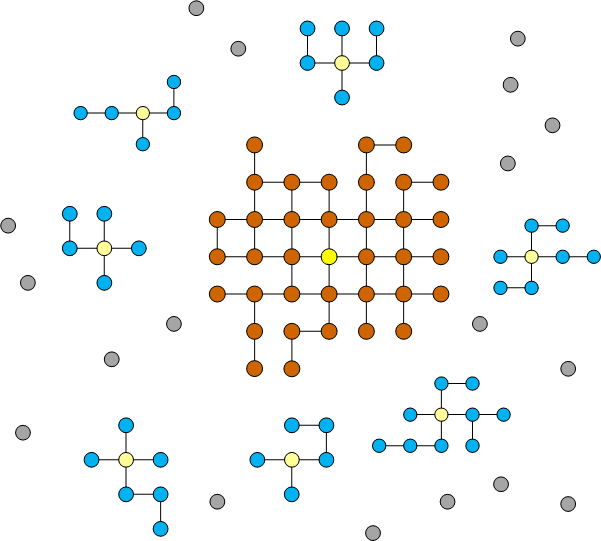
\includegraphics[scale=0.3]{slika-primer.png}
\caption{Vsako sliko opremi s podnapisom, ki pove, kaj slika prikazuje.}
\label{slika1}
\end{center}
\end{figure}

V to poglavje lahko tudi vključiš kakšen metodološko zanimiv del
kode. Primer vključitve kode oziroma implementirane funkcije v
programskem jeziku Python je:

\begin{lstlisting}
def fib(n):
    if n == 0:
        return 0
    elif n == 1:
        return 1
    else:
        return fib(n-1) + fib(n-2)
\end{lstlisting}

Izris te kode je lahko sicer tudi lepši, poskušaš lahko najti še
primernejši način vključevanja kode v Pythonu oziroma v tvojem izbranem
programskem jeziku v okolje \LaTeX{}.

\section{Rezultati}

V tem poglavju podaš rezultate s kratkim (enoodstavčnim)
komentarjem. Rezultate lahko prikažeš tudi v tabeli (primer je
tabela~\ref{tab1}).

Odstavke pri pisanju poročila v LaTeX-u ločiš tako, da pred novim
odstavkom pustiš prazno vrstico. Tudi, če pišeš poročilo v kakšnem
drugem urejevalniku, morajo odstavki biti vidno ločeni. To narediš z
zamikanjem ali pa z dodatnim presledkom.

\begin{table}[htbp]
\caption{Atributi in njihove zaloge vrednosti.}
\label{tab1}
\begin{center}
\begin{tabular}{llp{3cm}}
\hline
ime spremenljivke & definicijsko območje & opis \\
\hline
cena & [0, 500] & cena izdelka v EUR\\
teža & [1, 1000] & teža izdelka v dag \\
kakovost & [slaba|srednja|dobra] & kakovost izdelka \\
\hline
\end{tabular}
\end{center}
\end{table}

Podajanje rezultati naj bo primerno strukturirano. Če ima naloga več
podnalog, uporabi podpoglavja. Če bi želel poročati o rezultatih
izčrpno in pri tem uporabiti vrsto tabel ali grafov, razmisli o
varianti, kjer v tem poglavju prikažeš in komentiraš samo glavne
rezultate, kakšne manj zanimive detajle pa vključite v prilogo (glej
prilogi~\ref{app-res} in~\ref{app-code}).

\section{Izjava o izdelavi domače naloge}
Domačo nalogo in pripadajoče programe sem izdelal sam.

\appendix
\appendixpage
\section{\label{app-res}Podrobni rezultati poskusov}

Če je rezultatov v smislu tabel ali pa grafov v nalogi mnogo,
predstavi v osnovnem besedilu samo glavne, podroben prikaz
rezultatov pa lahko predstaviš v prilogi. V glavnem besedilu ne
pozabi navesti, da so podrobni rezultati podani v prilogi.

\section{\label{app-code}Programska koda}

Za domače naloge bo tipično potrebno kaj sprogramirati. Če ne bo od
vas zahtevano, da kodo oddate posebej, to vključite v prilogo. Čisto
za okus sem tu postavil nekaj kode, ki uporablja Orange
(\url{http://www.biolab.si/orange}) in razvrščanje v skupine.


\begin{lstlisting}
import random
import Orange

data_names = ["iris", "housing", "vehicle"]
data_sets = [Orange.data.Table(name) for name in data_names]

print "%10s %3s %3s %3s" % ("", "Rnd", "Div", "HC")
for data, name in zip(data_sets, data_names):
    random.seed(42)
    km_random = Orange.clustering.kmeans.Clustering(data, centroids = 3)
    km_diversity = Orange.clustering.kmeans.Clustering(data, centroids = 3,
        initialization=Orange.clustering.kmeans.init_diversity)
    km_hc = Orange.clustering.kmeans.Clustering(data, centroids = 3,
        initialization=Orange.clustering.kmeans.init_hclustering(n=100))
    print "%10s %3d %3d %3d" % (name, km_random.iteration, \
    km_diversity.iteration, km_hc.iteration)
\end{lstlisting}

\end{document}
